\section{Auswertung}
\label{sec:Auswertung}
\subsection{Funktionengenerator}
Zunächst wird das Signal des Funktionengenerators auf dem Osziloskop ausgegeben. Dort wird die Frequenz der gewählten Sinusfunktion auf 1 kHz justiert und eine Spannung von 52 mV gewählt. Anschließend wird der Aufbau wie in der Beschreibung beschrieben aufgebaut. Dabei werden die Filter der Frequenz entsprechend auf 1 kHz angepasst und die Verstärkung am Low-Pass Amplifier auf 200 eingestellt. Der Noise Generator wird zunächst einmal überbrückt indem er auf off gestellt wird.
\subsection{Phasenabhängigkeit der Ausgangsspannung}
Ziel des Teilversuchs ist es die Abhängigkeit der Ausgangsspannung $U_{\text{out}}$ von der Phasendifferenz $\phi$ der Eingangsspannung $U_{\text{sig}}$ und der Referenzsspannung $U_{\text{ref}}$ genauer zu untersuchen. Zunächst wird eine offset Messung der Phasenverschiebung der beiden Spannungen durchgeführt. Dafür wird der Phasenwinkel solange justiert bis ein Oszilloskopausschlag wie in Bild \ref{fig:phi0} erscheint, was einem Phasenwinkel von $\phi = 0^{\circ}$ entspricht.
\begin{figure}
  \centering
  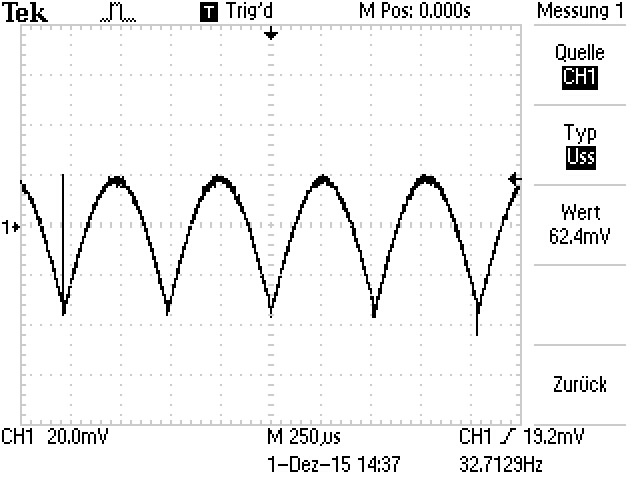
\includegraphics[height=5cm]{picture/1.JPG}
  \caption{$\phi = 0^{\circ}$ , offset Messung.}
  \label{fig:phi0}
\end{figure}
Daran wird die Phasenskala für den weiteren Versuchsverlauf ausgerichtet. Mittels eines Tiefpasses wird die Spannung, durch den Innenwiederstand integriert und die Zeitlich gemittelte Spannung auf einem Messgerät ausgegeben. Nach Berücksichtigung der Verstärkung ergibt sich nach Formel \ref{eqn:Uout} für eine Phasenverschiebung von $\phi = 0^{\circ}$ eine Spannung von
\begin{equation}
  U_{\text{out}} = \frac{2}{\pi} \cdot \frac{52 \cdot 10^{-3} \, V}{200} = 33.1 \cdot 10^{-3} \, V
  \label{eqn:Uout}
\end{equation}
Nach Formel ?? werden die theoretischen und praktischen Spannungswerte ausgerechnet und in Tabelle \ref{tab:Uphase} mit dem dazugehörigen Phasenwinkel aufgelistet.
\begin{table}
  \centering
  \begin{tabular}{c c c}
    \toprule
    $\phi$ & $U_{\text{theoretisch}}$ / $10^{-3} \cdot $ V & $U_{\text{praktisch}}$ / $10^{-3} \cdot $ V \\
    \midrule
    0	  &  33.1  &  32.5	\\
    30	&  28.6  &  27.5	\\
    60	&  16.5  &  12.5	\\
    90	&  0.0 	 &   2.5	\\
    120	& -16.5  & -17.5	\\
    150	& -28.6  & -30.0	\\
    180	& -33.1  & -35.0	\\
    210	& -28.6  & -27.5	\\
    240	& -16.5  & -12.5	\\
    270	&  0.0 	 &  2.5	 	\\
    300	&  16.5  &  17.5	\\
    330	&  28.6	 &  30.0	\\
  \end{tabular}
  \caption{$U_{\text{out}}$ bei verschiedenen Phasen.}
  \label{tab:Uphase}
\end{table}
Abbildung \ref{fig:Spannungsverlauf} kann man entnehmen das die Gemessene Spannung den Theoretischen Erwatungswert qualitativ erfüllt.
\begin{figure}
  \centering
  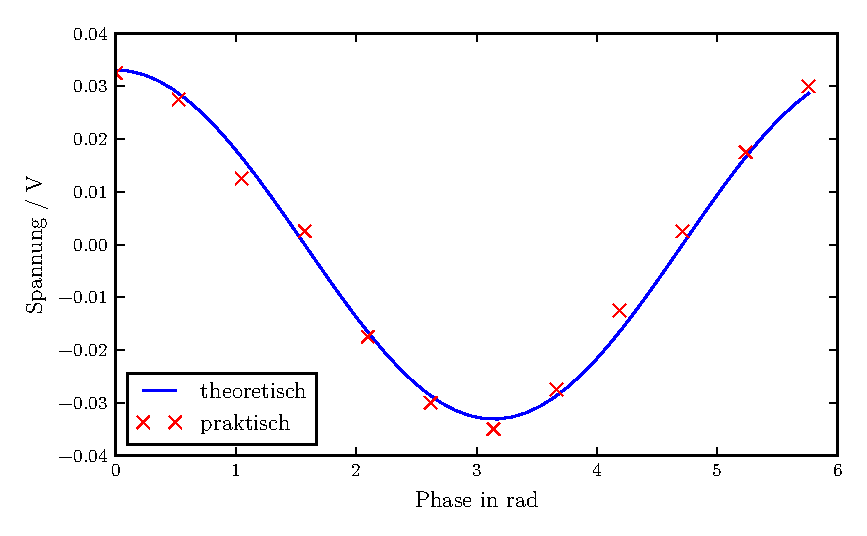
\includegraphics[height=5cm]{Spannungsverlauf.pdf}
  \caption{Spannungsverlauf}
  \label{fig:Spannungsverlauf}
\end{figure}
\subsection{Phasenabhängigkeit der Ausgangsspannung unter Einfluss einer Störfrequenz}
Für diesen Versuchsteil wird der Noisgenerator eingeschaltet. Dieser mischt Störfrequenzen der Gleichen Amplitude bei und erzeugt somit ein Stark verrauschtes Signal. Der Bandpass filtert schon ein Großteil der Störfrequenzen raus. Nach dem Mischen mit der Referenzspannung und der anschließenden Integration durch den Tiefpass, ergibt sich wieder eine zeitlich Konstante Spannung, falls der Integrationszeitraum hinreichend groß gewählt wurde. Die des Aufbaus entnommene Messwerte werden analog zum vorherigen Aufgabenteil ausgewertet und die Spannungen werden in Tabelle \ref{tab:Uphase2} ausgegeben und in Grafik \ref{fig:Spannungsverlauf} gegen die Phasenverschiebung aufgetragen.

\begin{table}
    \centering
    \begin{tabular}{c c c}
    	\toprule
    	$\phi$ & $U_{\text{theoretisch}}$ / $10^{-3} \cdot $ V & $U_{\text{praktisch}}$ / $10^{-3} \cdot $ V \\
    	\midrule
    	0   &  33.1  &  32.5        \\
    	30  &  28.6  &  27.5        \\
   	  60  &  16.5  &  10.0       \\
    	90  &  0.0   &   0.0        \\
    	120 & -16.5  & -17.5        \\
    	150 & -28.6  & -30.0        \\
    	180 & -33.1  & -35.0        \\
    	210 & -28.6  & -30.0        \\
    	240 & -16.5  & -15.0        \\
    	270 &  0.0   &  2.5         \\
    	300 &  16.5  &  17.5        \\
  	  330 &  28.6  &  30.0        \\
    	\end{tabular}
    \caption{$U_{\text{out}}$ bei verschiedenen Phasen.}
    \label{tab:Uphase2}
\end{table}

\begin{figure}
  \centering
  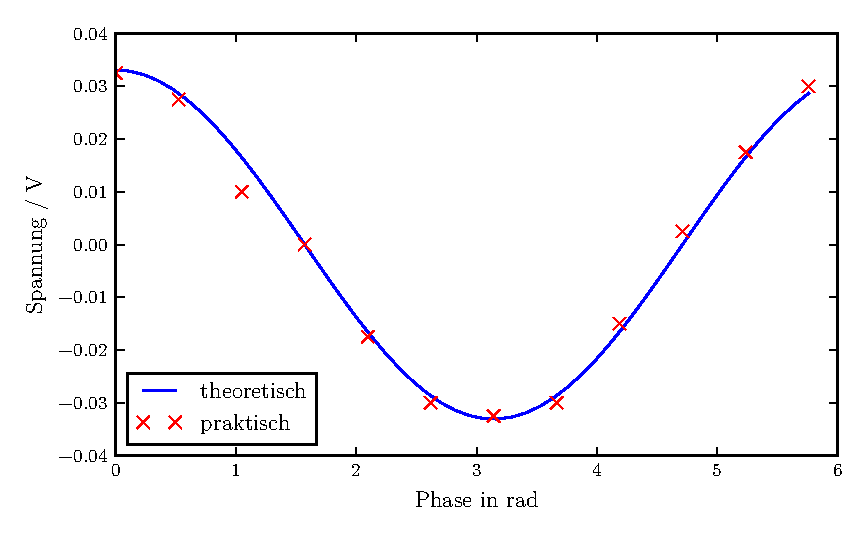
\includegraphics[height=5cm]{Spannungsverlauf2.pdf}
  \caption{Spannungsverlauf}
  \label{fig:Spannungsverlauf}
\end{figure}

Für die verschiedenen Phasen ergibt es durch die Multiplikation der Rechteckspannung mit der Sinusspannung verschiedene Graphen welche sich nach Formel \ref{eqn:foye} mittels einer Fourierentwicklung berrechnen lassen. Die zu den verschiedenen Phasen entsprechenden Graphen sind in Abbildung \ref{fig:graph1} und \ref{fig:graph2} zu sehen.

\begin{figure}
  \centering
  \begin{subfigure}{0.48\textwidth}
    \centering
    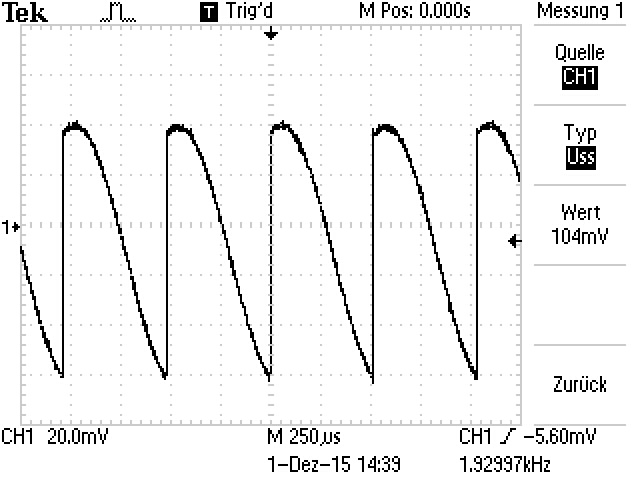
\includegraphics[height=5cm]{picture/2.JPG}
    \caption{$\phi = 60^{\circ}$}
  \end{subfigure}
  \begin{subfigure}{0.48\textwidth}
    \centering
    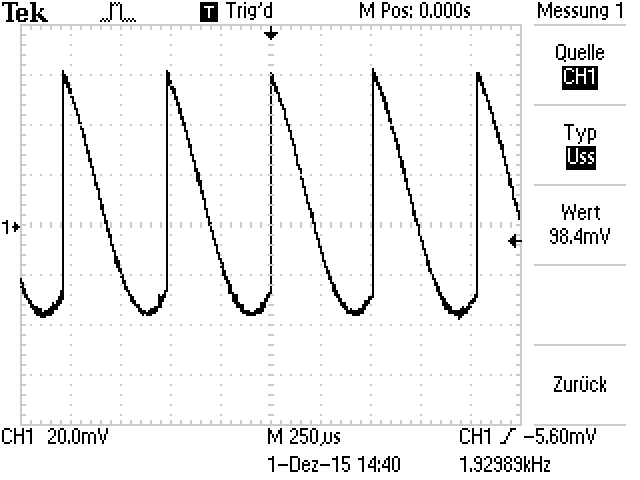
\includegraphics[height=5cm]{picture/3.JPG}
    \caption{$\phi = 120^{\circ}$}
  \end{subfigure}
  \caption{Fourierreihe für $60^{\circ}$ und $120^{\circ}$ Phasendifferenz}
  \label{fig:graph1}
\end{figure}
\begin{figure}
  \centering
  \begin{subfigure}{0.48\textwidth}
    \centering
    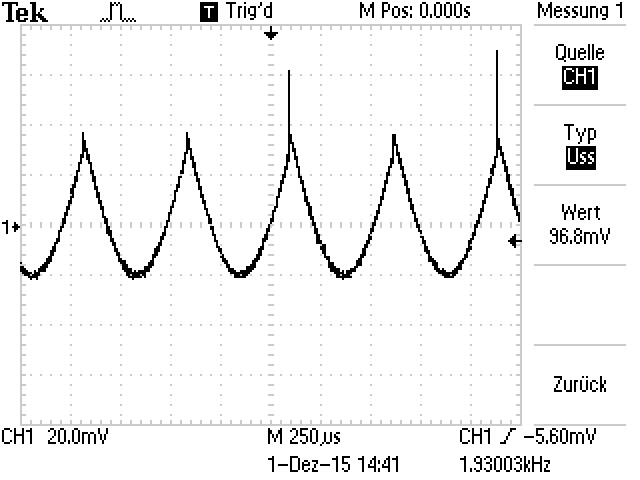
\includegraphics[height=5cm]{picture/4.JPG}
    \caption{$\phi = 180^{\circ}$}
  \end{subfigure}
  \begin{subfigure}{0.48\textwidth}
    \centering
    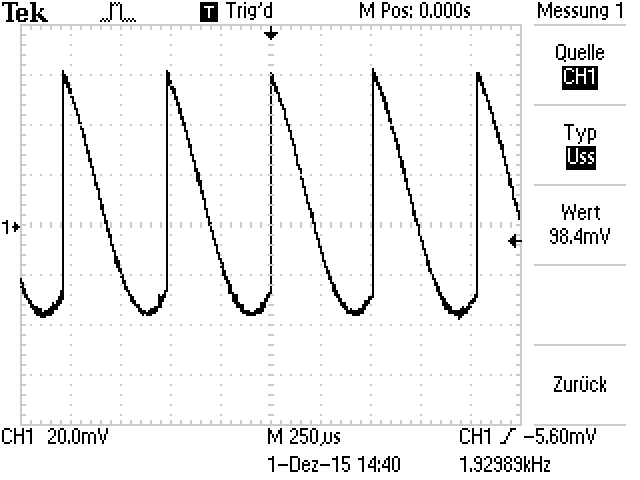
\includegraphics[height=5cm]{picture/3.JPG}
    \caption{$\phi = 240^{\circ}$}
  \end{subfigure}
  \caption{Fourierreihe für $180^{\circ}$ und $240^\circ$ Phasendifferenz}
  \label{fig:graph2}
\end{figure}


\subsection{Signal-Abstandsrealtion einer LED}
Aufgabe dieses Versuches ist die Signalstärke in Abhängigkeit des Abstandes zu messen. Der Lock-In-Verstärker dient dazu das durch die Umgebung verrauschte Signal zu filtern. Die LED wird mittels einer Rechteckspannung von 300 Hz betrieben. Durch justieren der Phasendifferenz soll die Spannung maximiert werden. Durch eine offset Messung, soll die Spannung der Photodiode vernachlässigt werden. Sie beträgt
\begin{equation}
  U_{offset}= \frac{-1}{1000} \, \text{V}
  \label{eqn:Uoffset}
\end{equation}
Die gemessenen Spannungen, deren Verstärkung und der Abstand $r$ sind in Tabelle \ref{tab:LED} aufgelistet. Dabei werden die gemessene Werte mit ihrer Verstärkung multipliziert und  die Offsetspannung von den Werten abgezogen.
\begin{equation}
  U_{\text{ber}} = \frac{U_{\text{out}}}{Gain} - \frac{U_{0}}{1000}
  \label{eqn:Uber}
\end{equation}

\begin{table}
  \centering
  \begin{tabular}{c c}
    \toprule
    $r$ / m & $U_\text(sig)$ / $10^{-4}$ \cdot V \\
    \midrule
    0.2  & 60.76	\\
    0.25 & 49.75	\\
    0.3  & 42.24	\\
    0.35 & 36.80	\\
    0.4  & 32.65	\\
    0.5  & 26.73	\\
    0.6  & 22.70	\\
    0.7  & 19.77	\\
    0.8  & 17.54	\\
    0.9  & 15.78	\\
    1.0  & 14.36	\\
    1.1  & 13.19	\\
    1.2  & 12.20	\\
    1.3  & 11.35	\\
    1.4  & 10.62	\\
    1.5  & 9.99		\\
    1.6  & 9.42		\\
    1.7  & 8.93		\\
    1.8  & 8.48		\\
    \bottomrule
  \end{tabular}
  \caption{Signalabstandsrelation}
  \label{tab:LED}
\end{table}
Mit Hilfe einer Fitfunktion wird eine Ausgleichsrechnung der Einzelnen Messpunkten durchgeführt. Die Koeffizienten der Ausgleichsgraden
\begin{equation}
  y = \alpha x + \beta
\end{equation}
sind,
\begin{eqnarray}
  \alpha = \num{-0.90 +- 0.07} \\
  \beta = \num{-6.55 +- 0.05}
  \label{eqn:Koef}
\end{eqnarray}
\begin{figure}
  \centering
  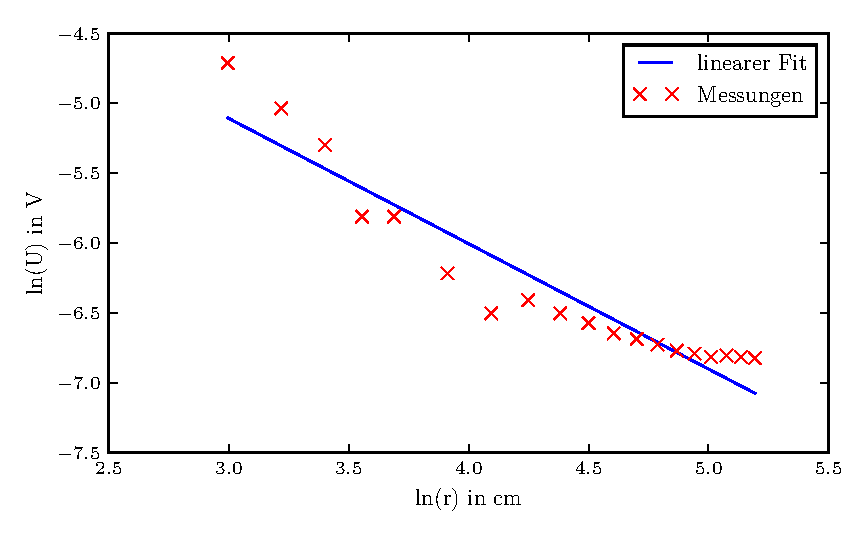
\includegraphics[height=5cm]{Abstand.pdf}
  \caption{Signalabstandsrelation}
  \label{fig:rU}
\end{figure}
